\chapter{Proteus is Turing Complete}\label{chapter:ProteusTC}

This section will describe how we will construct the proof showing that Proteus is TC.

\section{Useful information to be used in the proof}

First, I will discuss features about Proteus programs on a theoretical level.
Then, I will discuss features about the Proteus language that allow for the creation of a TM.
This is the background information that will guide the construction of the proof outline and ultimately the proof itself.

\subsection{Undecidable input}\label{subsec:UndecidableInput}

Because Proteus is a higher-level programming language, we can leverage the usage of Rice's Theorem, Theorem \ref{thm:RiceThm}.
Thus, given any input it is impossible to determine an answer to the Halting Problem.
Furthermore, one cannot determine if there is an actor that will be told to switch to a particular state.
With this knowledge, it is understood that any given Proteus program is undecidable.
Thus, I will look at how to create a TM in Proteus.

\subsection{Requirements of a TM}\label{subsec:ReqsofTM}

In this section, I will point out critical pieces of Proteus that prove useful to create a TM.
We can see that the core features to create a TM, seen previously in sections \ref{subsec:TMLogicalDesign} and \ref{subsubsec:ProgCalc}, include:
\begin{enumerate}
    \item Arithmetic and Logical Processing
    \item Memory storage and manipulation
    \item Conditional Logic
    \item Looping Logic
    \item Input/Output
\end{enumerate}

Recall the proteus grammar seen in section \ref{subsec:ProteusGrammar}.
I will now describe from the Proteus grammar how to construct/use Proteus creating each part of the TM.

\subsubsection{Arithmetic and Logical Processing}\label{subsubsec:ArithLogProc}

The grammar provides the following definitions for arithmetic and logical processing:
\begin{itemize}
    \item BinOp
    \item Type
    \item ConstExpr
\end{itemize}

'BinOp' handles all binary operations for both arithmetic and logical calculation.
Some features include addition, subtraction, multiplication, division, modular arithmetic, equivalence relations, and, and or.
Looking at brainfuck in section \ref{subsubsec:EsotericPL}, one can notice that the only necessary mathematical operations are addition and subtraction.
Furthermore, the only logical processing is seen in the looping mechanism.
If the value at the pointer is 0 and the input token is a '[', then the loop is skipped.
This means that there is an equality check which returns a boolean result.

Looking deeper at the types of Proteus, type consists of all the possible types that are built into the language:
\begin{itemize}
    \item int
    \item string
    \item boolean
    \item actorname
    \item statename
    \item eventname
\end{itemize}

Despite allowing for division, the set of integers is closed under truncation, which is how Proteus handles cases where normally it wouldn't be.
eg. 5 / 2 = 2.5, but under truncation 5 / 2 = 2.
These truncation rules are similar to those seen in other languages such as Java and C, \href{https://www.javatpoint.com/what-is-truncation-in-java}{in JAVA} \href{https://www.geeksforgeeks.org/trunc-truncf-truncl-c-language/}{in C}.

'ConstExpr' describes the 3 simple data types: Int, String, and Boolean.
These 3 types are capable of mimicking the behavior of brainfuck as well.

\subsubsection{Memory Storage and Manipulation}\label{subsubsec:MemStoManip}

The grammar provides the following definitions for memory storage and manipulation:
\begin{itemize}
    \item DefHSM
    \item DefState
    \item DefGlobalConst
    \item DecStmt
    \item AssignStmt
    \item SendStmt
\end{itemize}

'HSM' are Hierarchical State Machines which are actors in the language.
These state machines utilize states to determine logical processing.
These logical processes may utilize local or global variables that are stored, via the 'DecStmt' and 'DefGlobalConst' definitions respectively.

To modify data, the 'AssignStmt' was defined which allows for modifying the value of a given variable.
State Machines can modify state via the 'SendStmt' command.
Utilizing 'SendStmt', state machines can modify the state of themselves and other state machines as well.

\subsubsection{Conditional Logic}\label{subsubsec:CondLog}

The grammar provides the following definitions for conditional logic:
\begin{itemize}
    \item GoStmt
    \item JustGoStmt
    \item GoIfStmt
    \item ElseGoStmt
    \item IfStmt
\end{itemize}

Conditional Logic or Branching is necessary for a TM to compute any calculable function (see: Theorem \ref{thm:CTT}).
'GoStmt' is considered either a 'JustGoStmt' or a 'GoIfStmt', which are used to switch between states of a given HSM.
Similarly, the 'ElseGoStmt' switches to a particular state of a given HSM if the condition from the 'GoIfStmt' fails.

The 'IfStmt' is utilized for conditional logic within the processing of the state machines, and is akin to the standard if statements in other programming languages.
It is defined recursively to allow for nested "If ... else if.... else ..." statements.
These definitions allow for conditional statements to occur for a given HSM and within the code itself.

\subsubsection{Looping Logic}\label{subsubsec:LoopLog}

The only looping logic that can be seen in the garmmar that is built in, is the:
\begin{itemize}
    \item WhileStmt
\end{itemize}

This is the only necessary form of looping, as it can be broken by conditional statements and is capable of performing like other loops such as the do-while, for, and so forth.
This allows for more complex logical processing, such as recursion, which is a necessary requirement for TMs to perform any calculation.
A simplistic example of a problem that requires recursion would be the Ackermann Function.
See the definition of the Ackermann function here:
\[
\begin{aligned}
    A(0, n) &= n + 1\\
    A(m + 1, 0) &= A(m,1)\\
    A(m + 1, n + 1) &= A(m,\hspace{0.1cm} A(m + 1,n))
\end{aligned}
\]

Although being able to compute the Ackermann function requires recursion, it doesn't conclude that any system that can compute it is TC.
It was created to show that not all total computable functions are primitively recursive \cite{AckermannPR}.
The Ackermann function exists to show that not all functions can be represented with for loops, which is what primitive recursive functions are \cite{RecursiveFuncs}.
Nonetheless, all computable functions (regardless of their expression) are capable of being calculated by a TM, as stated by the Church-Turing Thesis (Theorem \ref{thm:CTT}).

\subsubsection{Input/Output}\label{subsubsec:IO}

Looking at the grammar definitions for:
\begin{itemize}
    \item Stmt
    \item PrintlnStmt
    \item PrintStmt
    \item SendStmt
\end{itemize}

From 'Stmt' I would like to highlight the 'SendStmt' command.
'SendStmt' is utilized to send events to a particular State Machine (i.e. an output).
By default, all actors are able to receive events.
'PrintlnStmt' and 'PrintStmt' are the standard print and println commands that are well known from other languages which serve as output to the console.
Although there is no explicit way to allow for input from the systems grammar dynamically, this is unnecessary as it can be preconfigured before runtime.
Thus, there exists a way to send inputs before the program is run via static input of values.

\section{Proteus Turing Machine Description}\label{sec:ProteusTMDescr}

By showing that any input to Proteus programs are undecidable and it is possible to create a TM in Proteus, Proteus can be shown to be TC.
This proof leverages the usage of both the Church-Turing Thesis, Theorem \ref{thm:CTT}, and Rice's Theorem, Theorem \ref{thm:RiceThm}.

I will explicitly create a TM using the built-in features seen previously in section \ref{subsec:ReqsofTM}.
After showing how to create a TM within Proteus, I will use Proteus to implement Conway's Game of Life and Rule 110 .
This is to demonstrate that the system is TC.
Recall demonstrating an implementation of CGoL or Rule110 indicates the system is TC from sections \ref{subsubsec:CGoL} and \ref{subsubsec:Rule110}.

\begin{enumerate}
    \item Define the set of internal states
    \item Define the initial state
    \item Define the final state
    \item Define the input alphabet
    \item Define the tape alphabet
    \item Define the state transitions
    \item Define the blank symbol
\end{enumerate}

A Proteus program will simulate the TM by having several parts.
The tape is a series of state machines, HSMs, that will be ordered as $c_{0}, c_{1}, \dots , c_{\text{n}}$ arbitrarily with $c_{\text{n}}$ being the last non-empty cell.
This order will be consistent and not allow state machines to swap places with each other in the sequence.
There will be an additional state machine which functions as the read/write head.
This state machine will be the one describing what the state of the TM and overall program is.
It contains a queue of events to be broadcast, with each entry in the queue containing a single event and target state machine.
Below is an image describing the system as a whole, followed by another image which shows the states and logical flow of the proposed TM.

\begin{figure}[h!]
    \centering
    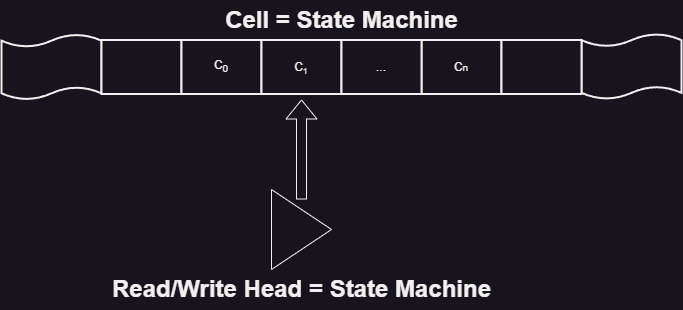
\includegraphics[width=16cm]{images/ProteusTMDesign.png}
       \caption{Design of TM in Proteus}
           \label{fig:ProteusTMDesign}
\end{figure}

When the Proteus program is run, the read/write head will enter the 'ProgramOn' State.
If the tape is empty, as in there are no state machines that are created by the programmer, then the read/write head enters the 'ProgramOff' state and halts.
If instead the cell is non-empty, then the read/write head enters the 'Read' state which begins the process of reading information from the tape.
If a write is to be issued, then the read/write head enter the 'Write' state and writes the new data in the current cell.
After the write, the read/write enters the 'Read' state once again.

The logic for movement to an adjacent cell is mirrored on the left and right sides.
I will describe the movement to the left-adjacent cell.
From the current cell, the read/write head enters the 'BoundLeft' state and determines whether it encounters another symbol or the blank.
If there is a symbol, then it still lies within the non-empty tape information and returns to the 'Read' state.
If instead there is a blank, this means that there is no state machine defined, and has extended past the bounds of the tape with given information.
The read/write head moves one cell to the right, then returns to the 'Read' state to continue processing.
Because Proteus does not allow for dynamic state machine creation, the read/write head leaves the blank unmodified along the tape.

To exit the program and enter the halting state, all state machines within the tape must enter the 'Off' state, indicated by the 'O' within Figure \ref{fig:ProteusStateTM}.
The read/write head enters the 'FindStart' state from the 'Read' state to prepare for halting.
In the 'FindStart' state, the read/write head will move to the left, one cell at a time.
When it encounters a blank cell, it moves the read/write head to the adjacent right cell and enters the 'Check' state.
In the check state, the read/write head moves one cell at a time to the right and checks if they are in the 'Off' state.
Upon encountering a cell that is not in the 'Off' state the read/write head enters the 'Read' state for further processing.
If every cell is in the 'Off' state, then the read/write head will encounter a blank on the next cell after $c_{\text{n}}$.
In this case, all state machines are in the 'Off' state and the read/write head enters the 'ProgramOff' state to halt.

Because the read/write head is itself a state machine, it contains an event queue for events to be broadcasted.
Each event is associated to a single state machine.
In order to find the proper state machine to send the event to, the read/write head must search for it within the bounds of the non-empty tape.
This searching cannot utilize 'FindStart', because if all state machines are off and there are some nonzero number of events still in the queue, then the machine will still have events to process, but end up in the 'ProgramOff' state.
As such, it must search for them and find them using an unoptimized algorithm such as brute forcing all possible movements across the non-empty tape.
Note that I will explicitly describe what values $x, y, \text{O}$ must be in the following section \ref{sec:Proof}.

\begin{figure}[h!]
    \centering
    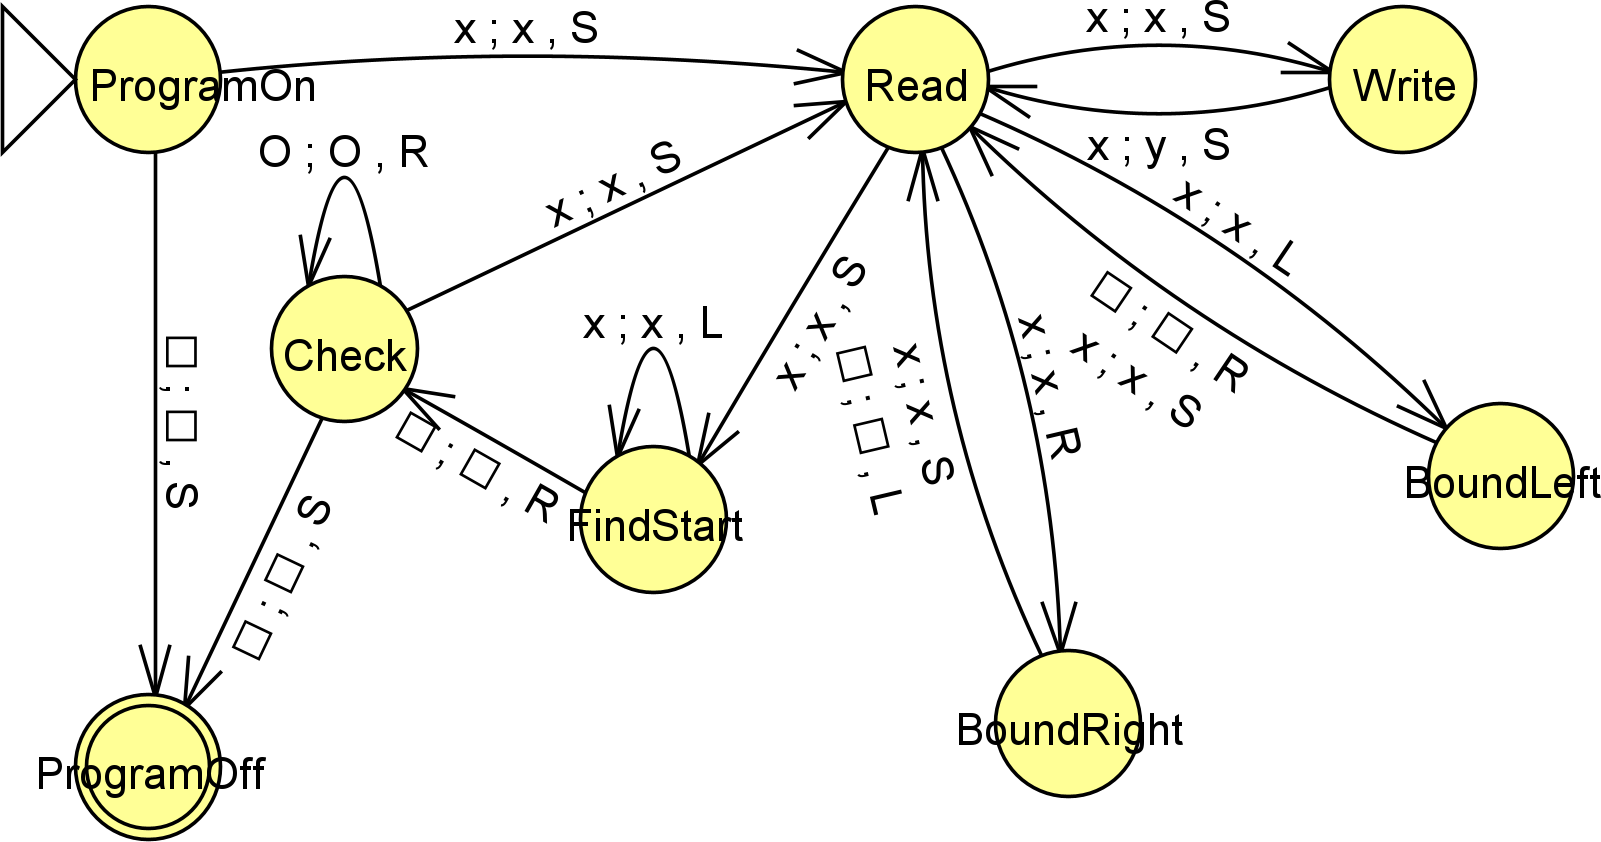
\includegraphics[width=16cm]{images/ProteusTM.png}
       \caption{TM State Diagram in Proteus}
           \label{fig:ProteusStateTM}
\end{figure}

\section{Definition of a Turing Machine in Proteus}\label{sec:DefnTMProteus}

To begin, I will describe the set of internal states of the TM, specifically of the state machine that is the read/write head.
There are two internal states that define the current status of the read/write head: 'ProgramOn' and 'ProgramOff'.
'ProgramOn' means that the program is currently running, while 'ProgramOff' means that the program has halted.
The read/write head also contains the following additional states:
\begin{itemize}
    \item Read state: Reads the current state of the cell at the read/write head.
    \item Send state: Broadcasts the event at the front of the event queue to the current cell.
    \item Move state: Moves the read/write head to the next/previous cell in the tape.
\end{itemize}
Let the set of internal states, be defined as follows:

\[
Q = \{\text{'ProgramOn'}, \text{'ProgramOff'}, \text{'Read'}, \text{'Send'}, \text{'Move'}\}
\]

$q_{0}$ is a state demonstrating that the program is currently running, i.e. the initial state.
To differentiate 'On' for the program (read/write head) versus the cell, the read/write head's initial state is defined as 'ProgramOn'.
Similarly, I named the final state of the Program as 'ProgramOff' for consistency.
Fis the set of halting states, and in this case contains only the element 'ProgramOff'.
Therefore, the initial state of the program and the halting state of the program can be described as:

\[
    \begin{aligned}
        q_{0} &= \text{'ProgramOn'} \\
        F &= \{\text{'ProgramOff'}\}
    \end{aligned}
\] 

The input alphabet consists of the symbols that appear as already existing on the tape.
Recall that each cell is a state machine in Proteus, seen in section \ref{sec:ProofOutline}.
The starting states for each cell (state machine) will be one of the following states: 'On' or 'Off'.
With this information we have the input alphabet:

\[
\Sigma = \{\text{'On'}, \text{'Off'}\}
\]

The symbols that can be written to and from the tape consist of the states within each state machine.
These are user defined, but also include the previously defined states: 'On' and 'Off'.
I will assume there is some number of states $n \in \mathbb{Z}_{\geq \text{0}}$ indicating that there are $0^{+}$ additional states designed for each state machine by the programmer.
Each state, $s_i$, are programmer created states which are not the 'On' or 'Off' states.
All states must output what the current state is of the state machine as a string.
This is to ensure that the read/write head is capable of knowing what state at the current location.
The last symbol to be included is the blank.
The blank represents that the cell has not changed state.
Thus, the list of symbols that can be written to and from the tape is as follows:

\[
\Gamma = \{\text{'On'}, \text{'Off'}, s_{0}, \dots, s_{n}, \raisebox{0.1cm}{\fbox{}}\} \text{ for } n \in \mathbb{Z}_{\geq \text{0}}
\]

The transition function is what allows the read/write head to change states.
In order to change the state of the overall program from 'ProgramOn' to 'ProgramOff' all internal state machines must be turned off.
This means that all non-blank cells on the tape must be in the 'ProgramOff' state.
Therefore, we can define transition states as:

DEFINE ALL THE TRANSITIONS FOR EACH OF THE INTERNAL STATES: READ, SEND, MOVE, PROGON, PROGOFF

\[
\delta = \text{hahahahaha}
\]

The blank symbol refers to a lambda transition, similar to those used in JFLAP (see section \ref{sec:TM} for information on JFLAP).
These blank symbols allow for transitioning between states without changing the internal state, or writing to the tape.

In summary, the following definitions create a TM for an arbitrary Proteus program:

\[
    \begin{aligned}
        Q &= \{\text{'ProgramOn'}, \text{'ProgramOff'}, \text{'Read'}, \text{'Send'}, \text{'Move'}\}\\
        F &= \{\text{'ProgramOff'}\}\\
        q_{0} &= \text{'ProgramOn'}\\
        \Sigma &= \{\text{'On'}, \text{'Off'}\}\\
        \Gamma &= \{\text{'On'}, \text{'Off'}, s_{0}, \dots, s_{n}, \raisebox{0.1cm}{\fbox{}}\} \text{ for } n \in \mathbb{Z}_{\geq \text{0}}
    \end{aligned}
\]

with the transition functions: 

\[
    \begin{aligned}
        \delta (q_{0}, 0) &= (q_{2}, 1, S),\\
        \delta (q_{0}, 1) &= (q_{1}, \raisebox{0.1cm}{\fbox{}}, R),\\
        \delta (q_{1}, 0) &= (q_{2}, 0, S),\\
        \delta (q_{1}, 1) &= (q_{0}, \raisebox{0.1cm}{\fbox{}}, R).\\
    \end{aligned}
\]

\section{Implementing Conway's Game of Life}\label{sec:ImplementCGoL}

Implementation of CGoL that is a demonstration of TC.

\section{Implementing Rule 110}\label{sec:ImplementRule110}

Implementation of Rule 110 that is a demonstration of TC.
